\documentclass[10pt,a4paper]{article}

\bibliographystyle{ieeetr}

\usepackage[margin=1in]{geometry}
\usepackage{graphicx}
\usepackage{subfig}
\usepackage{amsmath}
\usepackage{url}
\usepackage{pgfgantt}
\usepackage{pdfpages}
\usepackage[title]{appendix}

\graphicspath{{./figs/}}

\providecommand{\keywords}[1]{\textbf{\textit{Index terms---}} #1}
\newcommand{\code}[1]{\texttt{#1}}

\begin{document}

\begin{titlepage}
    \begin{center}

        \vspace*{2cm}
        
\includegraphics[width=.25\textwidth]{crest.png}

        \vspace*{1cm}
        {\Large \textbf{An Educational Kernel for the Raspberry Pi}} \\

        \vspace*{1cm}
        \textbf{Thomas Archbold} \\
        1602581 \\
        Department of Computer Science \\
        University of Warwick \\~\\

        April 29, 2019 \\~\\

        CS310 Third-year Project \\
        supervised by Adam Chester \\~\\

        \vfill

    \end{center}
\end{titlepage}

% abstract
% 1. Purpose
% 2. Methodology/Project Design 
% 3. Findings/Contribution
% 4. Research Limitations/Future work
% 5. Practical Implications/Conclusions

% No jargon - understand all terms without additional reading
\begin{abstract}
    This project presents an educational operating system for the Raspberry Pi 1
    Model B+, written for the purpose of demystifying aspects of operating
    systems development for the hobbyist programmer, especially with regards to
    low-level systems programming and core features to a computer's execution.
    It provides a small multiprocessing kernel developed with the aim of clarity
    of understanding and ease of extension. Together with a simple interface to
    further configure the system at compile-time, it aims to promote a practical
    approach to operating systems education. This interface can be easily
    extended to accommodate different models of inter-process communication.
    Future work should be aimed at increasing the operating system's usability
    in a real-world context, in particular with regard to user input and access
    to permanent storage, of which it has none. While it is limited in this
    sense, it provides a simple and open testbed on which to both study how key
    operating system concepts are implemented in practice, as well as invite the
    addition of new features.
\end{abstract}


\keywords{Operating systems, kernel, Raspberry Pi}

\tableofcontents

% introduction
% background
% motivational material

% main body:
%   design
%   methodology
%   development
%   results
%   testing
%   evaluation

% Author's Assessment of the Project
%   technical contribution of project
%   why considered relevant and important
%   how can others use it
%   why should it be considered an achievement
%   limitations of the project

\section{Introduction}
    Operating systems are some of the most pervasive pieces of software around,
    but due to their inherent complexity, their inner workings are often
    impenetrable to understand without specialist knowledge. While widespread
    access to a personal computer is nothing new, the introduction of the
    Raspberry Pi in recent years has rendered experimentation with computers
    much more affordable and hence readily available, inviting tinkering at all
    levels with less concern of economic loss. The Pi therefore provides an
    ideal platform for operating systems education -- novice developers looking
    to get involved in writing such systems have access to a standardised set of
    hardware that is inexpensive both to maintain and replace, if and when
    things go wrong. Now seven years since its initial release, the Raspberry
    Pi has several official operating systems to offer, each addressing its own
    issue such as ease-of-installation, Internet of Things integration, or
    classroom management \cite{OSes}, with many more unofficial ones. However,
    there is less in the way of those written to teach concepts of the operating
    system itself -- this project attempts to fill this gap by providing a
    configurable, educational operating system for the Raspberry Pi 1 Model B+,
    with a focus on presenting code which is simple to understand and providing
    clear interfaces to encourage ease of extensibility, and hence a practical,
    software-driven approach to learning about operating systems.

\subsection{Useful concepts}

% \section{Background}
\subsection{Motivation}
    An operating system draws together aspects from all over the field of
    computer science, whose development requires intimate knowledge of low-level
    concepts such as the computer's organisation and architecture, up to an
    understanding for the more abstract in designing how processes communicate
    or implementing filesystems. The opportunity to write one as part of this
    project was therefore appealing as it served not only to provide the author
    with experience in an area of computer science of great interest,
    but also the chance to unite and put into practice many of the topics
    learned throughout the undergraduate computer science course. One of the key
    motivations of this project was therefore to gain experience in low-level
    systems programming and interacting with real-world hardware, all the while
    creating a useful and entirely self-contained piece of software.

    The main goal of this project is to provide an operating system for the
    Raspberry Pi that is capable of booting on real hardware, for both
    educational and hobbyist use. An important aspect of this is gaining
    practical experience in this unique area of software development, and so in
    addition to being configurable at compile-time, offering multiple approaches
    to process scheduling and inter-process communication, it also aims to
    easily-understandable and open to extension. In order to achieve this it
    must also implement a basic interface to manage this compile-time
    configuration. Also key to the project's success is the ability to boot on
    real hardware - while it would largely be possible to implement in a solely
    emulated environment with the help of a virtual machine, this project
    attempts to provide the additional valuable experience of taking real-world
    design considerations and observing their effects on live hardware, the
    latter of which is easily ignored if working only through an emulator. 

\subsection{Relevant Material}
    To this end, there are a handful of modern resources for getting involved
    with operating systems development -- a particularly useful one at the time
    of first carrying out research for the project's proposal was
    \code{wiki.osdev.org}, which contains information about the creation of
    operating systems and acts as a community for hobbyist operating system
    developers. However, much of the focus is on the x86 platform and past
    providing a brief overview of the idiosyncrasies of the Raspberry Pi as well
    as the code to get a barebones kernel to boot, there is little material on
    the specifics required to get core systems working on the platform.
    Cambridge's \textit{Baking Pi} \cite{BakingPi} provides more help in this
    regard, with Alex Chadwick's comprehensive tutorials proving an invaluable
    resource for information such as accessing registers and peripherals
    specific to the Raspberry Pi. The project can, however, be much further
    extended to guide through the implementation of core operating system
    concepts such as memory management, the process model, interprocess
    communication, and filesystems. Another aspect in which this series of
    tutorials diverges with the goal of this project is the language in which it
    has been implemented -- while assembly is an undeniably language in which to
    be competent, it is not the most easily-understandable, in stark contrast to
    what this project hopes to achieve. The resource which aligns most tightly
    with the aim of this project is \cite{jsandler}, whose tutorials have served
    as an outline to how many key features of the project have been implemented.
    
    Finally, other notable resources which are in place to teach general
    operating systems development are Stanford's \textit{Pintos} \cite{Pintos}
    and Tanenbaum's MINIX operating system; the former was written to accompany
    the university's CS140 Operating Systems course, while the latter is an
    illustrative operating system written alongside the book \textit{Operating
    Systems: Design and Implementation} \cite{MINIX}, showing how features are
    implemented in practice. Helin and Renberg's \textit{The Little Book About
    OS Development} \cite{littleosbook} also serves as a guide to writing one's
    own operating system. The only drawback to these three is their focus on the
    x86 architecture, and while they are useful resources it is in concept only,
    given the gap which was found to quickly form from focusing on a different
    processor.

\subsection{Why is this project worthwhile?}
    The project is worthwhile firstly as it provides an accessible gateway into
    systems programming and operating systems development. Given the relative
    difficulty and additional effort required to get involved with this area of
    software development as opposed to others, for example by reading technical
    reference manuals and building an intimate knowledge of the hardware with
    which you are working, it therefore finds its use in easing this transition
    and making the learning curve associated with its involvement less
    intimidating and more approachable. In doing this, the project is also
    worthwhile in that it demystifies some of the key considerations that go
    into operating system implementations, not only in high-level concepts such
    as processes, but also the low-level with notions such as memory-mapped I/O
    and the processor's registers. In providing this opportunity to see theory
    in practice, it further opens up the opportunity for experimentation and
    invites practical self-learning, and hopefully clarifying why existing
    operating systems work the way they do.

    While the current background material has similar aims, this project
    addresses the gap that is left unfilled by them, by tackling a different
    architecture, and thus forms one more part in the ecosystem of operating
    systems education.

% \input{sections/motivational}
\input{sections/conclusions}

\bibliography{bibliography}

\begin{appendices}
%
%    \pagenumbering{gobble}
%
%    % Revised Timetable
%    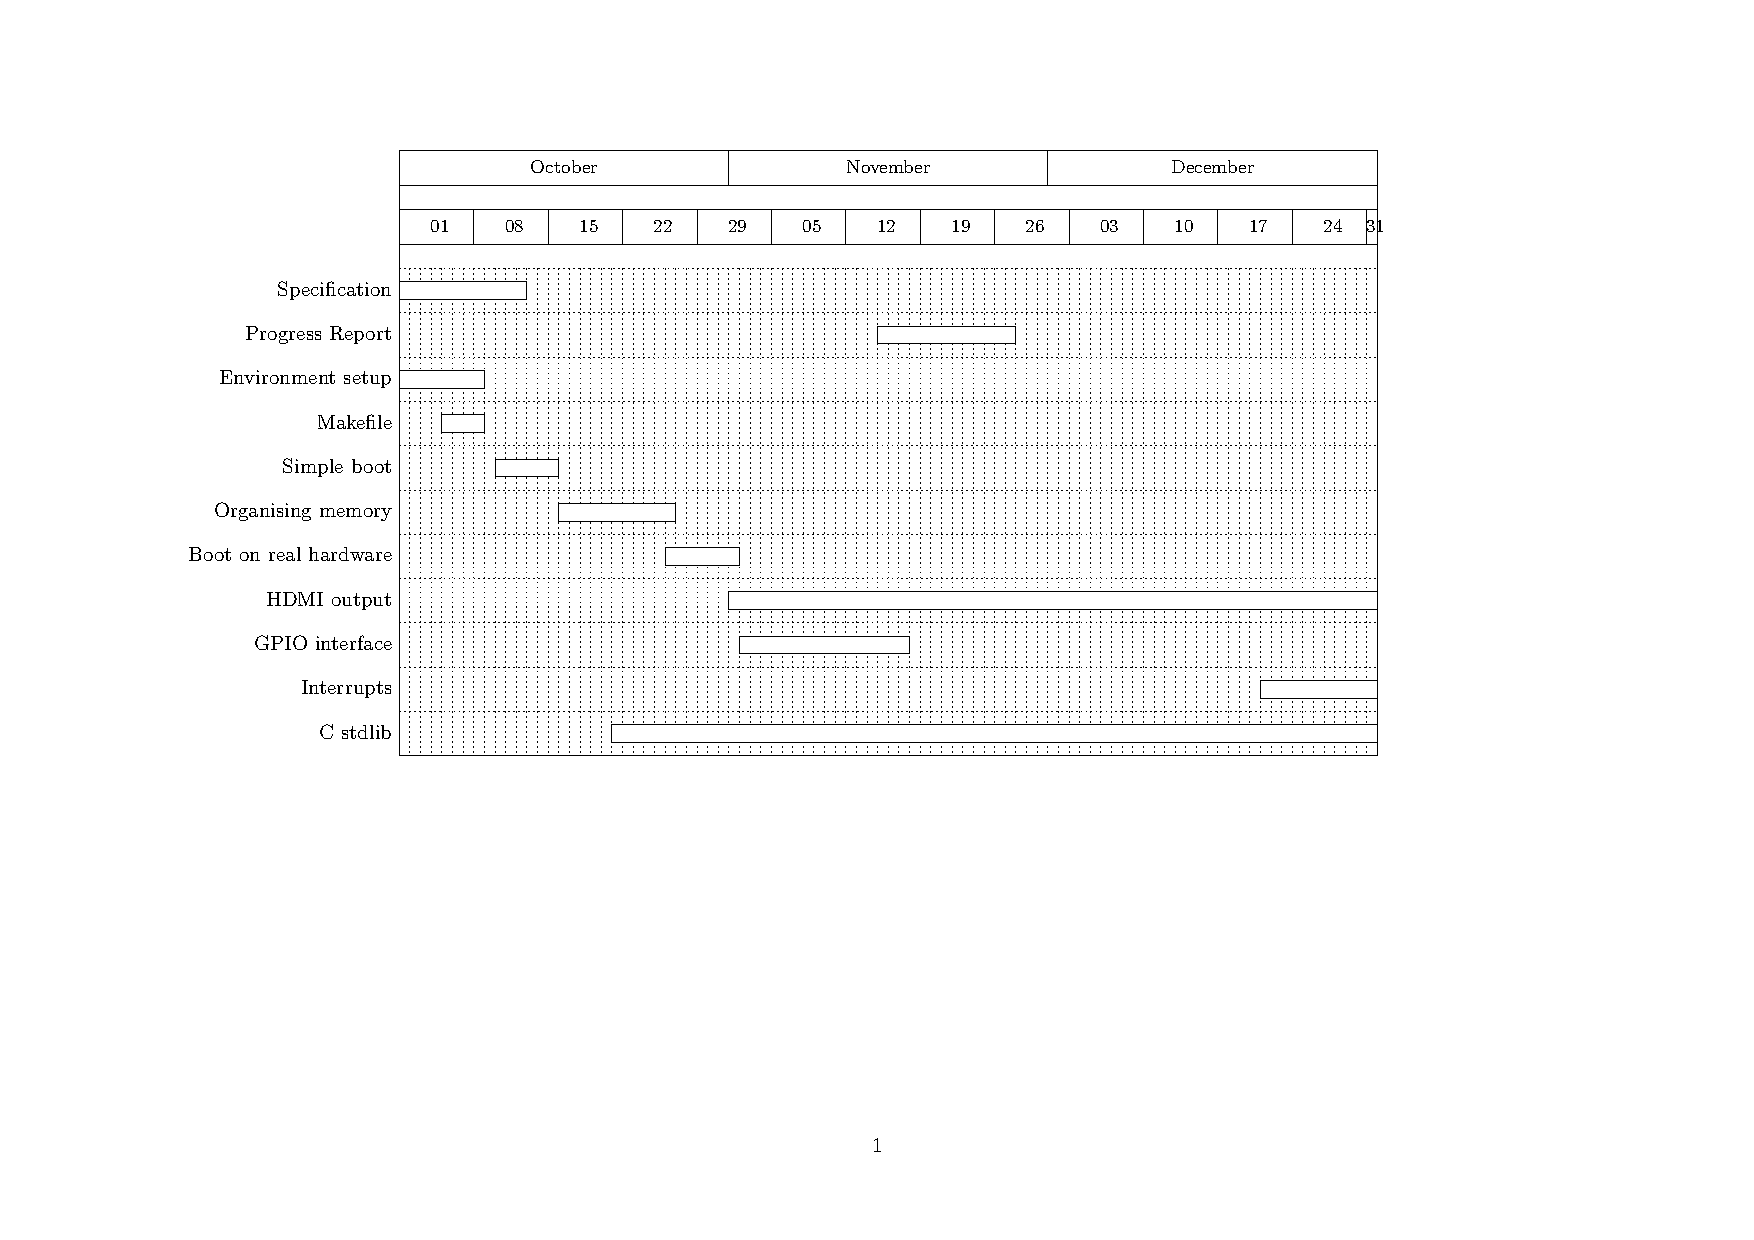
\includepdf[landscape=true,pages=1,pagecommand={\section{Revised Timetable}}]{timetable/timetable.pdf}
%    \includepdf[landscape=true,pages=2,pagecommand={}]{timetable/timetable.pdf}
%
%    % Project Specification
%    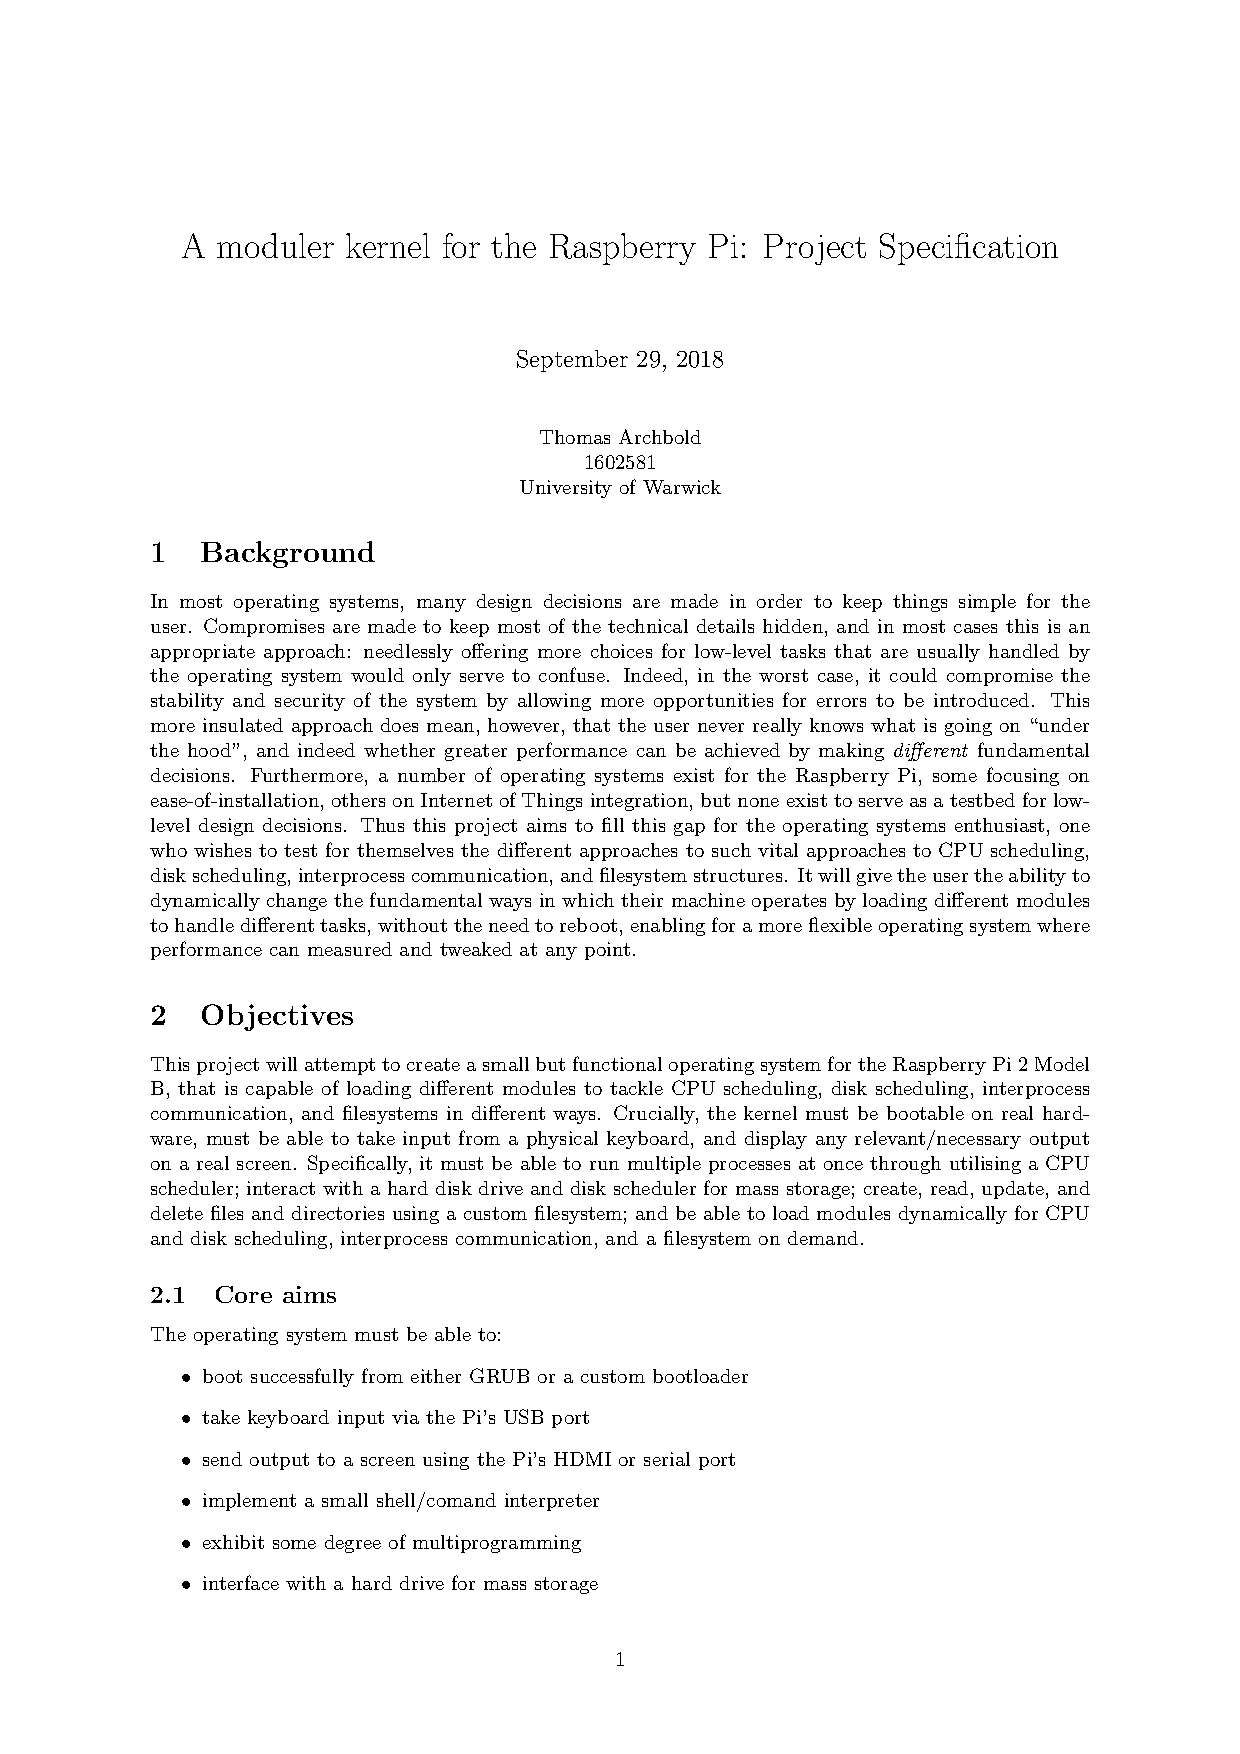
\includepdf[pages=1,pagecommand={\section{Project Specification}}]{../specification/specification.pdf}
%    \includepdf[pages=2-6,pagecommand={}]{../specification/specification.pdf}
%    \includepdf[landscape=true,pages=7-,pagecommand={}]{../specification/specification.pdf}
%
\end{appendices}

\end{document}
